% Insert after Section 3; no document environment is included.
% Preamble: \usepackage{amsmath,booktabs,tabularx,graphicx,hyperref}
% The recommendation image is stored in figures/section4/ beside this source.
% Compile from docs/ so figures/section4/ resolves correctly.
% Sources: the shared Section 4 Google Doc; backend grading/recommendation code;
% docs/evaluation.md; docs/validation/MVP-checks-2026-10-30.md.
% Checkpoint: main, dbbe536. Tests/screenshots are supplied historical evidence;
% no new live-provider run or participant study was performed for this revision.

\section{Advanced Component: Prototype and Evaluation}
\label{sec:advanced}

\subsection{Selected Direction and Integration into the Product}
The project combines Direction~4, Automated Assessment, and Direction~2,
Personalised Learning Paths and Recommendations, in the Writing Clinic.
The cycle connects Task~2 submission, feedback, teacher review, targeted
practice, revision and a new-topic task. The assessment contribution is
rubric-based grading with validation and review; the recommendation
contribution is explainable activity selection from learner evidence.

At commit \texttt{dbbe536}, these are integrated services with persistent
state rather than isolated AI calls. Results are linked to immutable
revisions and versioned grading configurations. Teacher confirmation and
publication are separate steps: only current, accepted and released
evidence contributes to the official skill profile. Objective answer-key
grading is a separate accepted source, not an exception that makes AI
output official.

\subsection{AI-Assisted Writing Assessment Prototype}
Submission pins the assignment version and preserves paragraph identifiers.
An identical resubmission of the latest content reuses its revision; changed
content creates a new revision when limits permit. Each grading run pins
the rubric, prompt and provider/model configuration for traceability.

The validator requires one score per criterion, valid ranges and permitted
skill identifiers. It computes the weighted overall score rounded to
0.5 bands and rejects an inconsistent supplied overall band. Local findings
must quote text present in the cited revision paragraph; the backend
computes offsets. Global observations may have no local anchors.
Invalid output, refusals and incomplete responses are recorded without
creating a valid assessment from that failed attempt. Quote existence
establishes an anchor, not the correctness of the judgment.

Validated output passes review-routing heuristics: an essay below 100 words,
missing findings, selected instruction-like phrases, or a criterion spread
above three bands triggers a flag. These rules are not calibrated accuracy
or academic-integrity detectors. Unflagged practice feedback may be shown
provisionally under the release policy; graded or flagged results await
teacher review. Missing AI configuration routes the submission to manual
review without inventing scores.

Assigned instructors claim cases and enter criterion scores, explanations,
findings and skill observations. AI bands are not automatically adopted as
teacher decisions. Confirmation preserves the AI result and records a
separate decision and audit event; version checks reject stale updates.
Publication follows the assignment policy. Corrections and appeals retain
decision history. Self-review is prohibited, and the administrator role
alone does not grant grading permission. Live-provider scoring remains
unverified; the seeded teaching rubric also requires expert review before
accuracy evaluation.

\subsection{Explainable Recommendation Prototype}
The profile uses current accepted, published evidence. For each
attempt--skill pair, only the latest applicable revision contributes,
preventing revisions from counting as independent opportunities.
Observed outcomes map to 1 (met), 0.5 (partial) or 0 (not met).
Unobserved outcomes are excluded; absent evidence produces unknown strength.
Three observed opportunities form an experimental support threshold,
not a calibrated mastery probability.

Candidates are published, accessible items in actively enrolled courses.
Completed lessons are excluded; practice targets must satisfy publication,
opening-time, late-submission and attempt-quota rules. Skill prerequisites
are checked, with an explicit exception for diagnostic tags. Eligible
candidates use the experimental ranking:
\[
 S_i=0.60N_i+0.25D_i+0.15F_i,
\]
where $N_i$ is skill need weighted by curriculum coverage, $D_i$ is
difficulty fit to the target band, and $F_i$ rewards activities outside
the five most recent attempts. Unknown strength receives a provisional
need of 0.7 before coverage weighting. Up to three items are selected,
preferring different target skills. Stored profile/policy versions,
candidates, score components and template reasons make choices traceable.
The weights and explanations have not been independently validated.

\begin{figure}[htbp]
\centering
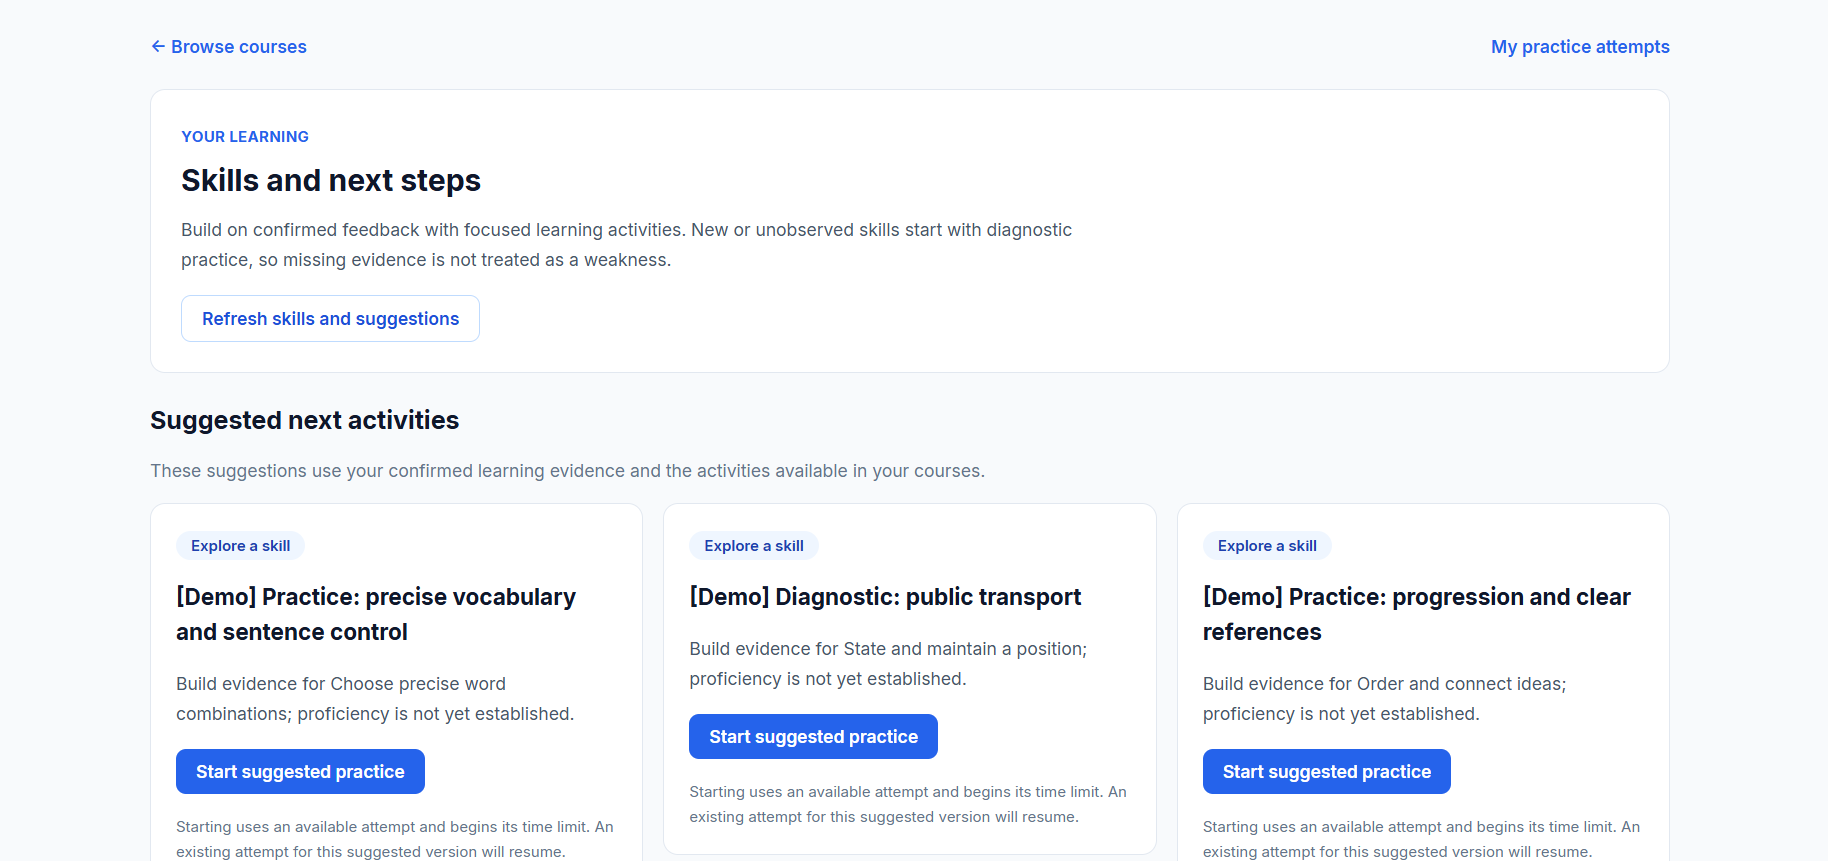
\includegraphics[width=\linewidth]{figures/section4/recommendations.png}
\caption{Supplied recommendation view for unobserved skills. The reasons
state that proficiency is not yet established; this demonstrates the
unknown-evidence case rather than validated recommendation relevance.}
\label{fig:recommendation-unknown}
\end{figure}

\subsection{Initial Results and Evaluation Plan}
The recorded checkpoint has 133 passing regular backend tests and
19 separately passing PostgreSQL integration tests; provider calls in tests
are mocked. Supplied UI screenshots illustrate selected prototype states.
Synthetic evaluation replay checks the tooling, not scoring accuracy or
learning gains. Detailed software checks are reported in
Section~\ref{sec:quality}.

\begin{center}
\begingroup\small
\begin{tabularx}{\linewidth}{@{}p{0.31\linewidth}X@{}}
\toprule
\textbf{Evidence} & \textbf{Current conclusion} \\
\midrule
Automated rule/integration tests & Tested validation, review, publication and policy behaviour; no claim of exhaustive correctness. \\
Selected UI screenshots & Prototype screens are illustrated; a repeatable full three-role browser run remains to be verified. \\
Synthetic evaluation replay & Evaluation pipeline executes; no expert accuracy or learning-effect evidence. \\
Live AI and expert judgments & Accuracy, latency, recommendation relevance and teacher-effort studies remain pending. \\
\bottomrule
\end{tabularx}
\endgroup
\end{center}

\paragraph{Assessment evaluation.}
Collect an initial 20--30 permitted essays with independent expert labels
under a reviewed rubric. Keep original essays and revisions in the same
development/held-out group; freeze model, prompt and rubric before holdout.
Compare the proposed pipeline with a declared simple structured-prompt
baseline using the same model and rubric. Report overall/per-criterion MAE
alongside attempted/valid/failed coverage, errors above one overall band,
quote-anchor validity, and measured latency and tokens. Missing predictions
count as failures; MAE on valid outputs must not hide them. Expert review
will assess finding correctness and teacher effort separately. MAE
$\leq 0.5$ is a proposed target, not an achieved result.

\paragraph{Recommendation evaluation.}
Export actual policy choices and compare fixed-curriculum and
lowest-criterion baselines on the same eligible candidate snapshot.
Collect independent expert relevance labels and report precision at the
returned count, number returned and invalid targets; overlap alone is
descriptive. Learning gains require a separate participant study using
targeted practice, revision and a new-topic task. Remaining risks are
expert/data availability, provider cost and variability, small samples and
untuned policy weights. The reproducible protocol is documented in
\href{https://github.com/huyho44/IELTS-Evaluator-Pro/blob/dbbe536/docs/evaluation.md}{the evaluation guide}.
